\chapter{Summary and future work}\label{ch:conclusion} % 7

As single-assignment languages and Kahn process networks demonstrate,
monotonicity can serve as the foundation of diverse
deterministic-by-construction parallel programming models.  The LVars
programming model takes monotonicity as a starting point and
generalizes single assignment to monotonic multiple assignment,
parameterized by a lattice.  The LVars model, and the accompanying
LVish library, \either{support my claim}{demonstrate} that lattice-based data structures are
a general and practical unifying abstraction for deterministic and
quasi-deterministic parallel \either{and distributed}{} programming.

\ifdefined\DISSERTATION
\section{Another look at the deterministic parallel landscape}
\fi

Let us reconsider how LVars fit into the deterministic parallel
programming landscape that we mapped out in \either{Chapter}{Section}~\ref{ch:intro}:
\begin{itemize}
  \item \emph{No-shared-state parallelism:} The purely functional core
    of the $\lambdaLVar$ and $\lambdaLVish$ calculi (and of the LVish
    Haskell library) allow no-shared-state, pure task parallelism.  Of
    course, shared-state programming is the point of the LVars model.
    However, it is significant that we take pure programming as a
    starting point, because it distinguishes the LVars model from
    approaches such as DPJ that begin with a
    parallel (but nondeterministic) language and then restrict the
    sharing of state to regain determinism.  The LVars model works in
    the other direction: it begins with a deterministic parallel
    language without shared state, and then adds limited effects that
    retain determinism.
  \item \emph{Data-flow parallelism:} As we have seen, because LVars
    are lattice-generic, the LVars model can subsume Kahn process
    networks and other parallel programming models based on data flow,
    since we can use LVars to represent a lattice of channel
    histories, ordered by a prefix ordering.
  \item \emph{Single-assignment parallelism:} Single-assignment
    variables, or IVars, are also subsumed by LVars: an IVar is an
    LVar whose lattice has one ``empty'' state and multiple ``full''
    states (where $\forall{i}.\; \mathit{empty} < \mathit{full_i}$).
    In fact, given how useful IVars are, the subsumption of IVars by
    LVars demonstrates that immutability is an important special case
    of monotonicity.\footnote{As Neil Conway puts it, ``Immutability
      is a special case of monotone growth, albeit a particularly
      useful one''
      (\url{https://twitter.com/neil_conway/status/392337034896871424}).}
  \item \emph{Imperative disjoint parallelism:} Although the LVars
    model generally does \emph{not} require that the state accessed by
    concurrent threads is disjoint, this style of ensuring determinism
    is still compatible with the LVars model, and it is practically
    achievable using the @ParST@ monad transformer in LVish, as we saw
    in Section~\ref{s:lvish-disjoint}.
\end{itemize}

In addition to subsuming or accommodating all these existing points on
the landscape, we have identified a new class of
\emph{quasi-deterministic} programs and developed a programming model
that supports quasi-determinism by construction.  A
quasi-deterministic model allows programs that perform \emph{freezing}
and are deterministic modulo write-after-freeze exceptions.  The
ability to freeze and read the exact contents of an LVar greatly
increases the expressiveness of the LVars model, especially when used
in conjunction with event handlers.  Furthermore, we can regain full
determinism by ensuring that freezing happens last, and, as we saw in
Section~\ref{subsection:lvish-regaining-full-determinism-with-runparthenfreeze},
it is possible to enforce this ``freeze after writing'' requirement at
the implementation level.

Of course, there is still more work to do.  For example, although
imperative disjoint parallelism and the LVars model seem to be
compatible, as evidenced by the use of @ParST@ in LVish, we have not
yet formalized their relationship.  In fact, this is an example of a
general pattern in which the LVish library is usually one step ahead
of the LVars formalism: to take another example, the LVish library
supported the update operations of
Section~\either{\ref{subsection:lvars-generalizing-from-least-upper-bound-writes}}{\ref{s:lvars-generalizing}}
(which are commutative and inflationary but not necessarily
idempotent) well before the notion had been formalized in
$\lambdaLVish$.  Moreover, even for the parts of the LVish library
that \emph{are} fully accounted for in the model, we do not have proof
that the library is a faithful implementation of the formal LVars
model.

Although it is unlikely that this game of catch-up can ever be won, an
interesting direction to pursue for future work would be a
\emph{verified} implementation of LVish, for instance, in a
dependently typed programming language.  Even though a fully verified
implementation of LVish (including the scheduler implementation) is an
ambitious goal, a more manageable first step might be individually
verified LVar data structures, implemented in a dependently typed
language such as Coq or Agda.  The type system of such a language is
rich enough to express properties that must be true of an LVar, such
as that the states that it can take on form a lattice and that writes
are commutative and inflationary.

\ifdefined\DISSERTATION
\begin{figure}[h]
  \vspace{-1em}
  \begin{center}
    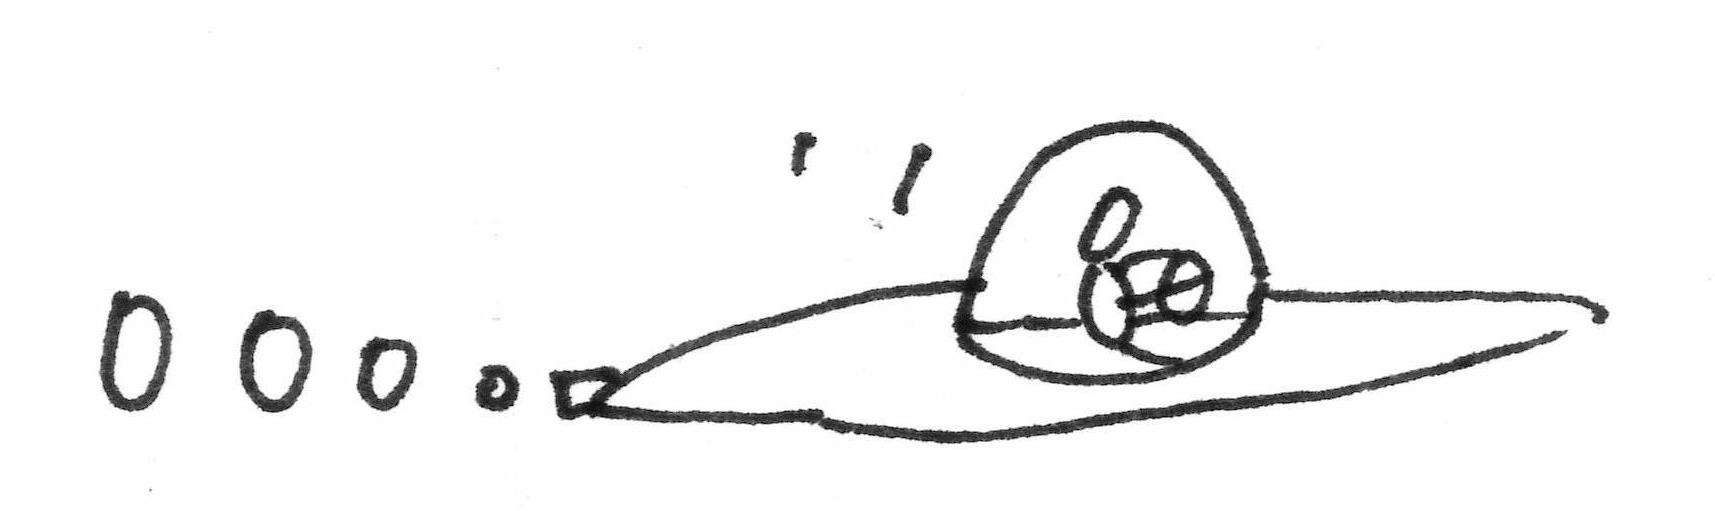
\includegraphics[scale=0.15]{../illustrations/flying-saucer}
  \end{center}
  \vspace{-1em}
\end{figure}
\fi

\ifdefined\DISSERTATION
\section{Distributed programming and the future of LVars and LVish}

Most of this dissertation concerns the problem of how to program
\emph{parallel} systems, in which programs are running on multiple
processors.  However, I am also concerned with the problem of how to
program \emph{distributed} systems, in which programs must run on
networked computers around the world.  Enormous bodies of work have
been developed to deal with both of these problems, and one of the
roles that programming languages research can play is to try to find
unifying abstractions between the two. It is in that spirit that I
have explored the relationship of LVars to existing work on
distributed systems.

LVars are a close cousin to convergent replicated data types
(CvRDTs)~\cite{crdts,crdts-tr}, which leverage lattice properties to
guarantee that all replicas of an object (for instance, in a
distributed database) are eventually consistent.
Chapter~\ref{ch:distributed} begins to explore the relationship
between LVars and CvRDTs by porting LVar-style threshold reads to the
CvRDT setting, but there is much more work to do here.  Most
immediately, although the idea of a single lattice-based framework for
reasoning about both strongly consistent and eventually consistent
queries of distributed data is appealing and elegant, it is not yet
clear what the compelling applications for threshold-readable CvRDTs
are.

As a further step, it should also be possible to ``back-port'' ideas
from the realm of CvRDTs to LVars.  In fact, support for
not-necessarily-idempotent updates to LVars was inspired in part by
CvRDTs, which have always permitted arbitrary inflationary and
commutative writes to individual replicas (the lub operation is only
used when replicas' states are \emph{merged} with one another).  The
LVars model might further benefit from techniques pioneered in the
work on CvRDTs to support data structures that allow seemingly
non-monotonic updates, such as counters that support decrements as
well as increments and sets that support removals as well as
additions~\cite{crdts}.

Finally, existing work on CvRDTs, as well as the work on distributed
lattice-based programming languages like Bloom~\cite{bloom-cidr,
  blooml}, may serve as a source of inspiration for a future version
of LVish that supports distributed execution.
\fi
